\section{Hardware Overview}
\label{hw_sec}

This section describes the hardware setup needed for enabling Android Open ADK on STM32-based kits. In particular, STEVAL-MKI062V2 (iNEMO) \cite{STM_inemo} board has been used in this demo application, but the work presented can be easily adapted to whatever STM32 based board. The STEVAL-MKI062V2 is the second generation of the iNEMO module family. It combines accelerometers, gyroscopes and magnetometers with pressure and temperature sensors to provide 3-axis sensing of linear, angular and magnetic motion, complemented with temperature and barometer/altitude readings, offering in this way a 10 degrees of freedom (DOF) platform. More specifically, the board integrates five STMicroelectronics sensors: a 2-axis roll-and-pitch gyroscope, a 1-axis yaw gyroscope, a 6-axis geomagnetic module, a pressure sensor, and a temperature sensor (see {\bf Figure \ref{fig:inemov2}}).

\begin{center}
	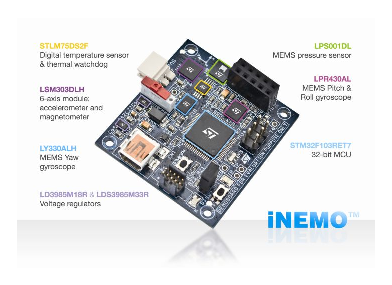
\includegraphics[width=0.95\linewidth]{pics/inemov2.eps}
	\captionof{figure}{iNEMO V2 platform.}
	\label{fig:inemov2}
\end{center}

As we said, the communication between the board and the Android device is realized using the Android Open ADK: according to this protocol the iNEMO acts as the USB host (powers the bus and enumerates devices) and the Android-powered device acts as the USB device (see section \ref{adk_sec} for more details). Since the iNEMO does not natively integrate a USB port, it is necessary to use a USB Host Shield in order to provide USB Host functionality to the board. In this work it has been used the USB Host Shield furnished by Sparkfun\footnote{Sparkfun USB Host Shield: \url{http://www.sparkfun.com/products/9947}}, but whatever equivalent board offering Maxim MAX3421E\cite{max3421e} USB host controller can be adopted. The iNEMO board communicates with the Host Shield through a Serial Peripheral Interface (SPI) bus: as a matter of fact, the Extended Connector (J8) of the iNEMO provides an SPI interface and 4 GPIOs (see {\bf Figure \ref{fig:j8}}) that can be used to control the Shield.

\begin{center}
	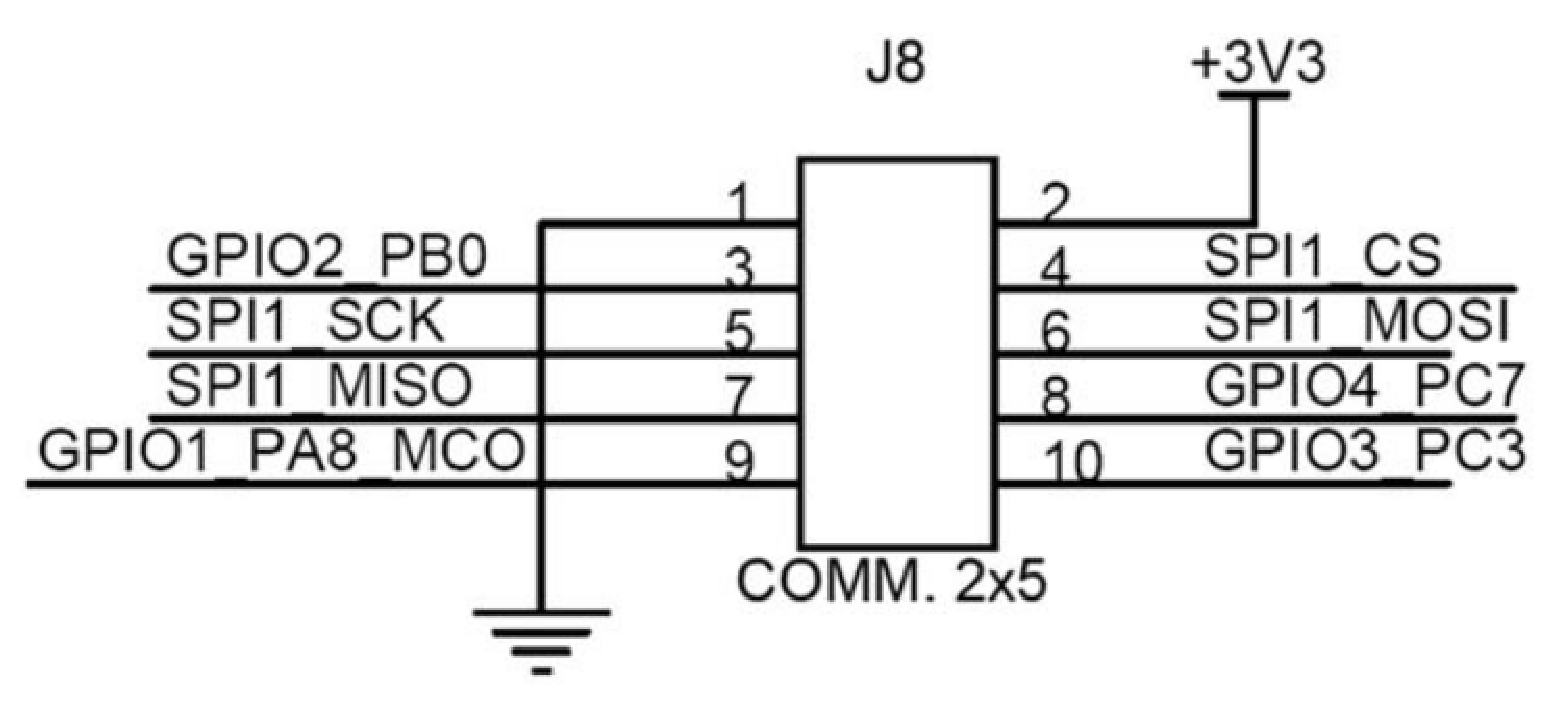
\includegraphics[width=0.95\linewidth]{pics/j8.eps}
	\captionof{figure}{Extended Connector (J8) schematic.}
	\label{fig:j8}
\end{center}

The connections between the iNEMO board and the USB Host Shield are shown in {\bf Figure \ref{fig:spi}}. This picture shows also that the Shield must be powered by means of an external power supply (9V) on VIn pin.

\begin{center}
	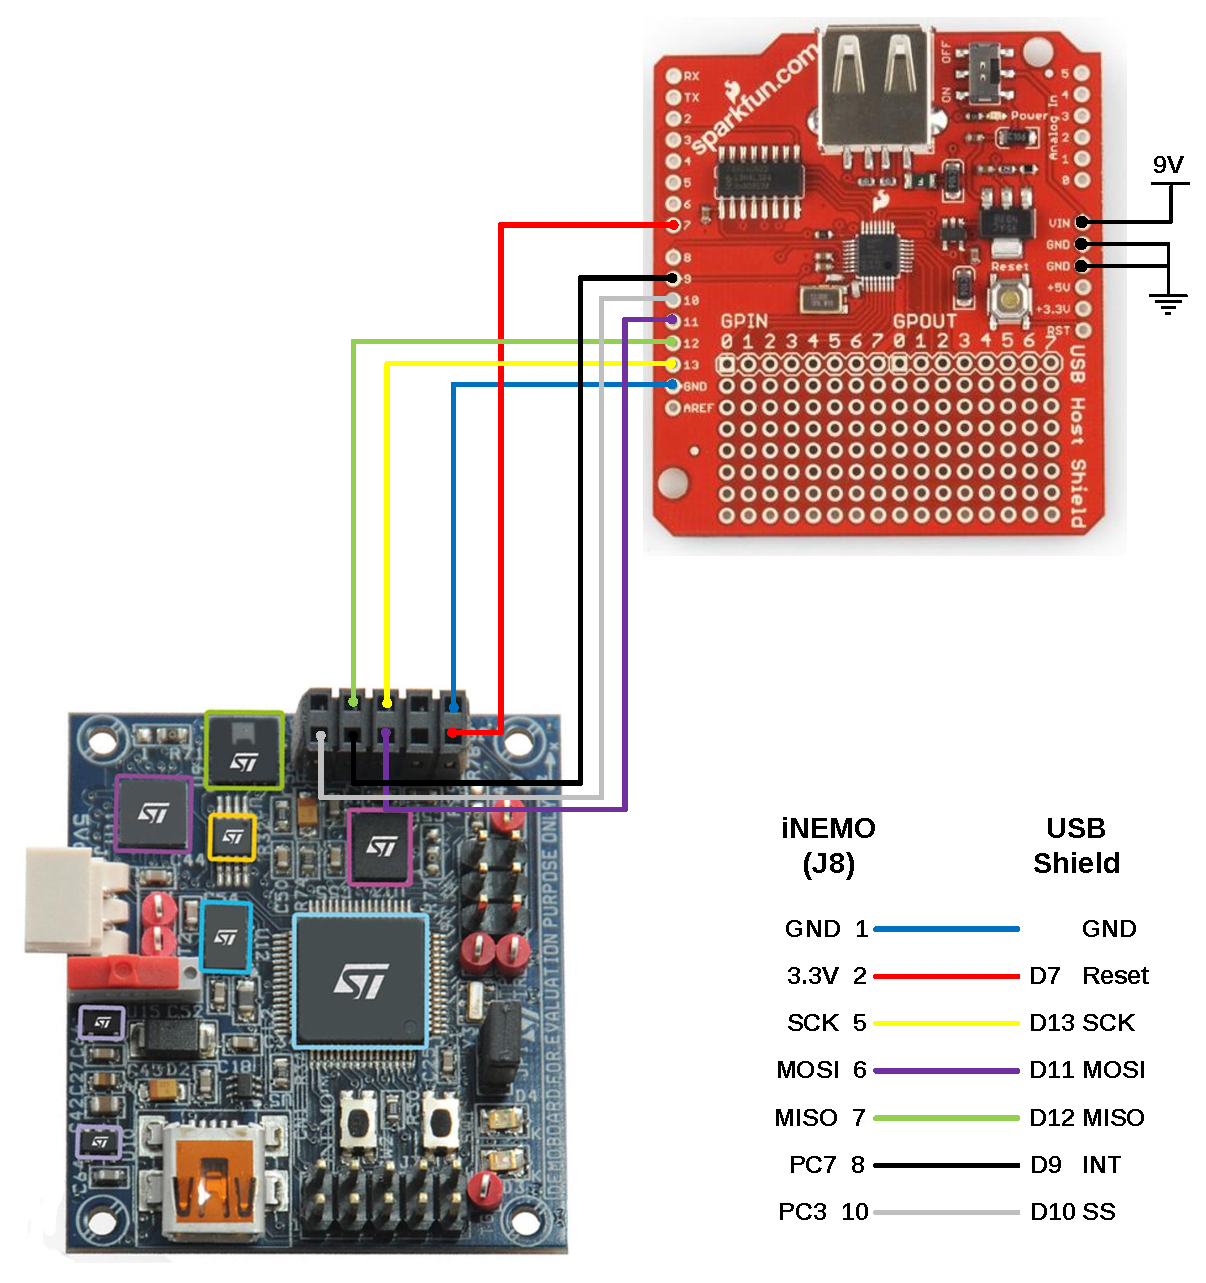
\includegraphics[width=0.95\linewidth]{pics/SPI_wirings.eps}
	\captionof{figure}{Connections between the iNEMO board and the USB Host Shield.}
	\label{fig:spi}
\end{center}

For debugging purposes, a TTL-232R-PCB by FTDI\cite{ttl232r} has been connected to the 6-pin COM J4 connector of the iNEMO board.

{\bf Figure \ref{fig:connections}} shows an overview of the components used in this work and the connections between them.

\begin{center}
	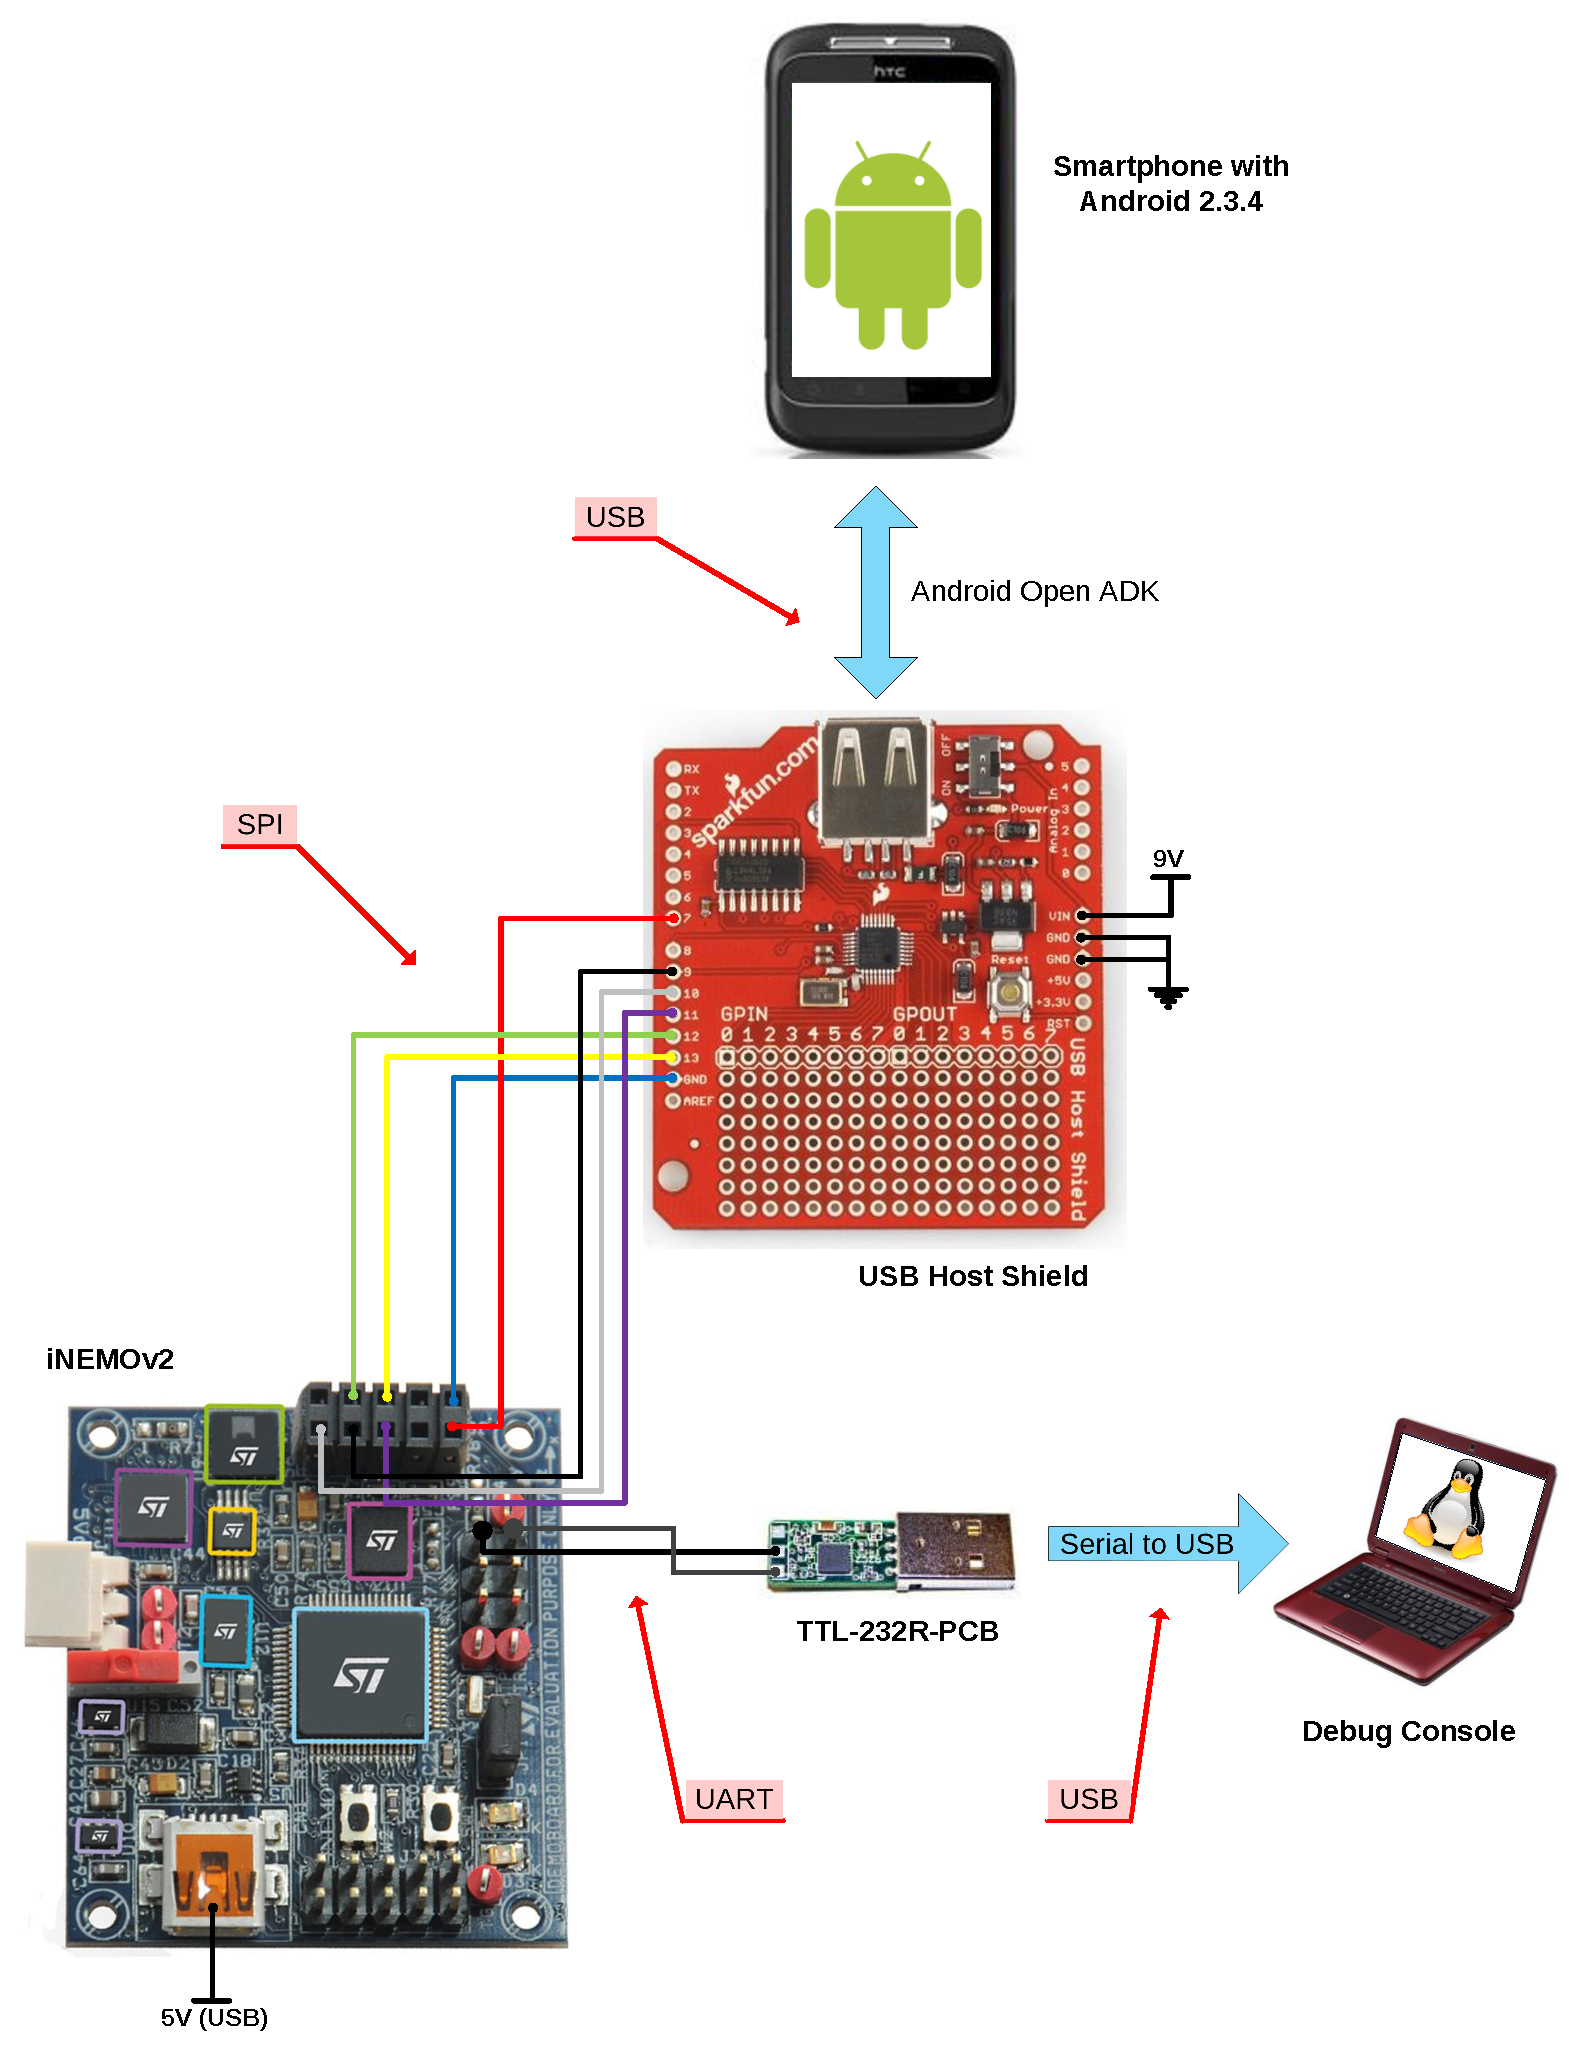
\includegraphics[width=0.95\linewidth]{pics/connections.eps}
	\captionof{figure}{Overview of the hardware used.}
	\label{fig:connections}
\end{center}

